\chapter{pyNE 3.0 - General Usage}
\label{Chap:GeneralUsage}

\lettrine[lines=2]{\color{myBrown}\textsf{T}}{}his chapter serves as a brief introduction to the pyNE\footnote{\textbf{py}thon \textbf{N}ano\textbf{E}lectronics} data acquisition software (V3.0). This quick-start guide will cover the basic structure of the software. For a full list of available instruments, functions and measurement ranges, please refer to Section 2: Instruments, Functions and Ranges. For information on installation, please refer to Section 3: Installation and Setup.\\

\section{Basic layout of the \textit{control file}}
The \textit{control file} lays out the entire measurement procedure intended by the user. It can be written from scratch quite quickly, but we recommend you save frequently used files in your own private folder for more rapid/efficient usage.\\
\\
Note: We currently use the \textit{Spyder} IDE\footnote{Integrated development environment} to edit and execute these files. It may run, but has not been tested, in other IDEs. CTRL+C stops the execution of a running script and thus serves as an emergency stop button.\\
\\
The \textit{control file} has a structure in which the desired measurement routine is described. Figure~\ref{Fig:SimpleControl} outlines this for the simple scenario of a single source-drain measurement performed by a Keithley~2401. In the header, Lines~9-11, we import all the required functions from the main pyNE directory, most of these are handled by import.py. As part of this, one needs to specify the current working directory, which is done in Line~10. This needs to be edited for the given installation.\\

\begin{verbatim}
os.chdir('D:\Python\PyNE_3p0\')
\end{verbatim}

\begin{figure}[h]
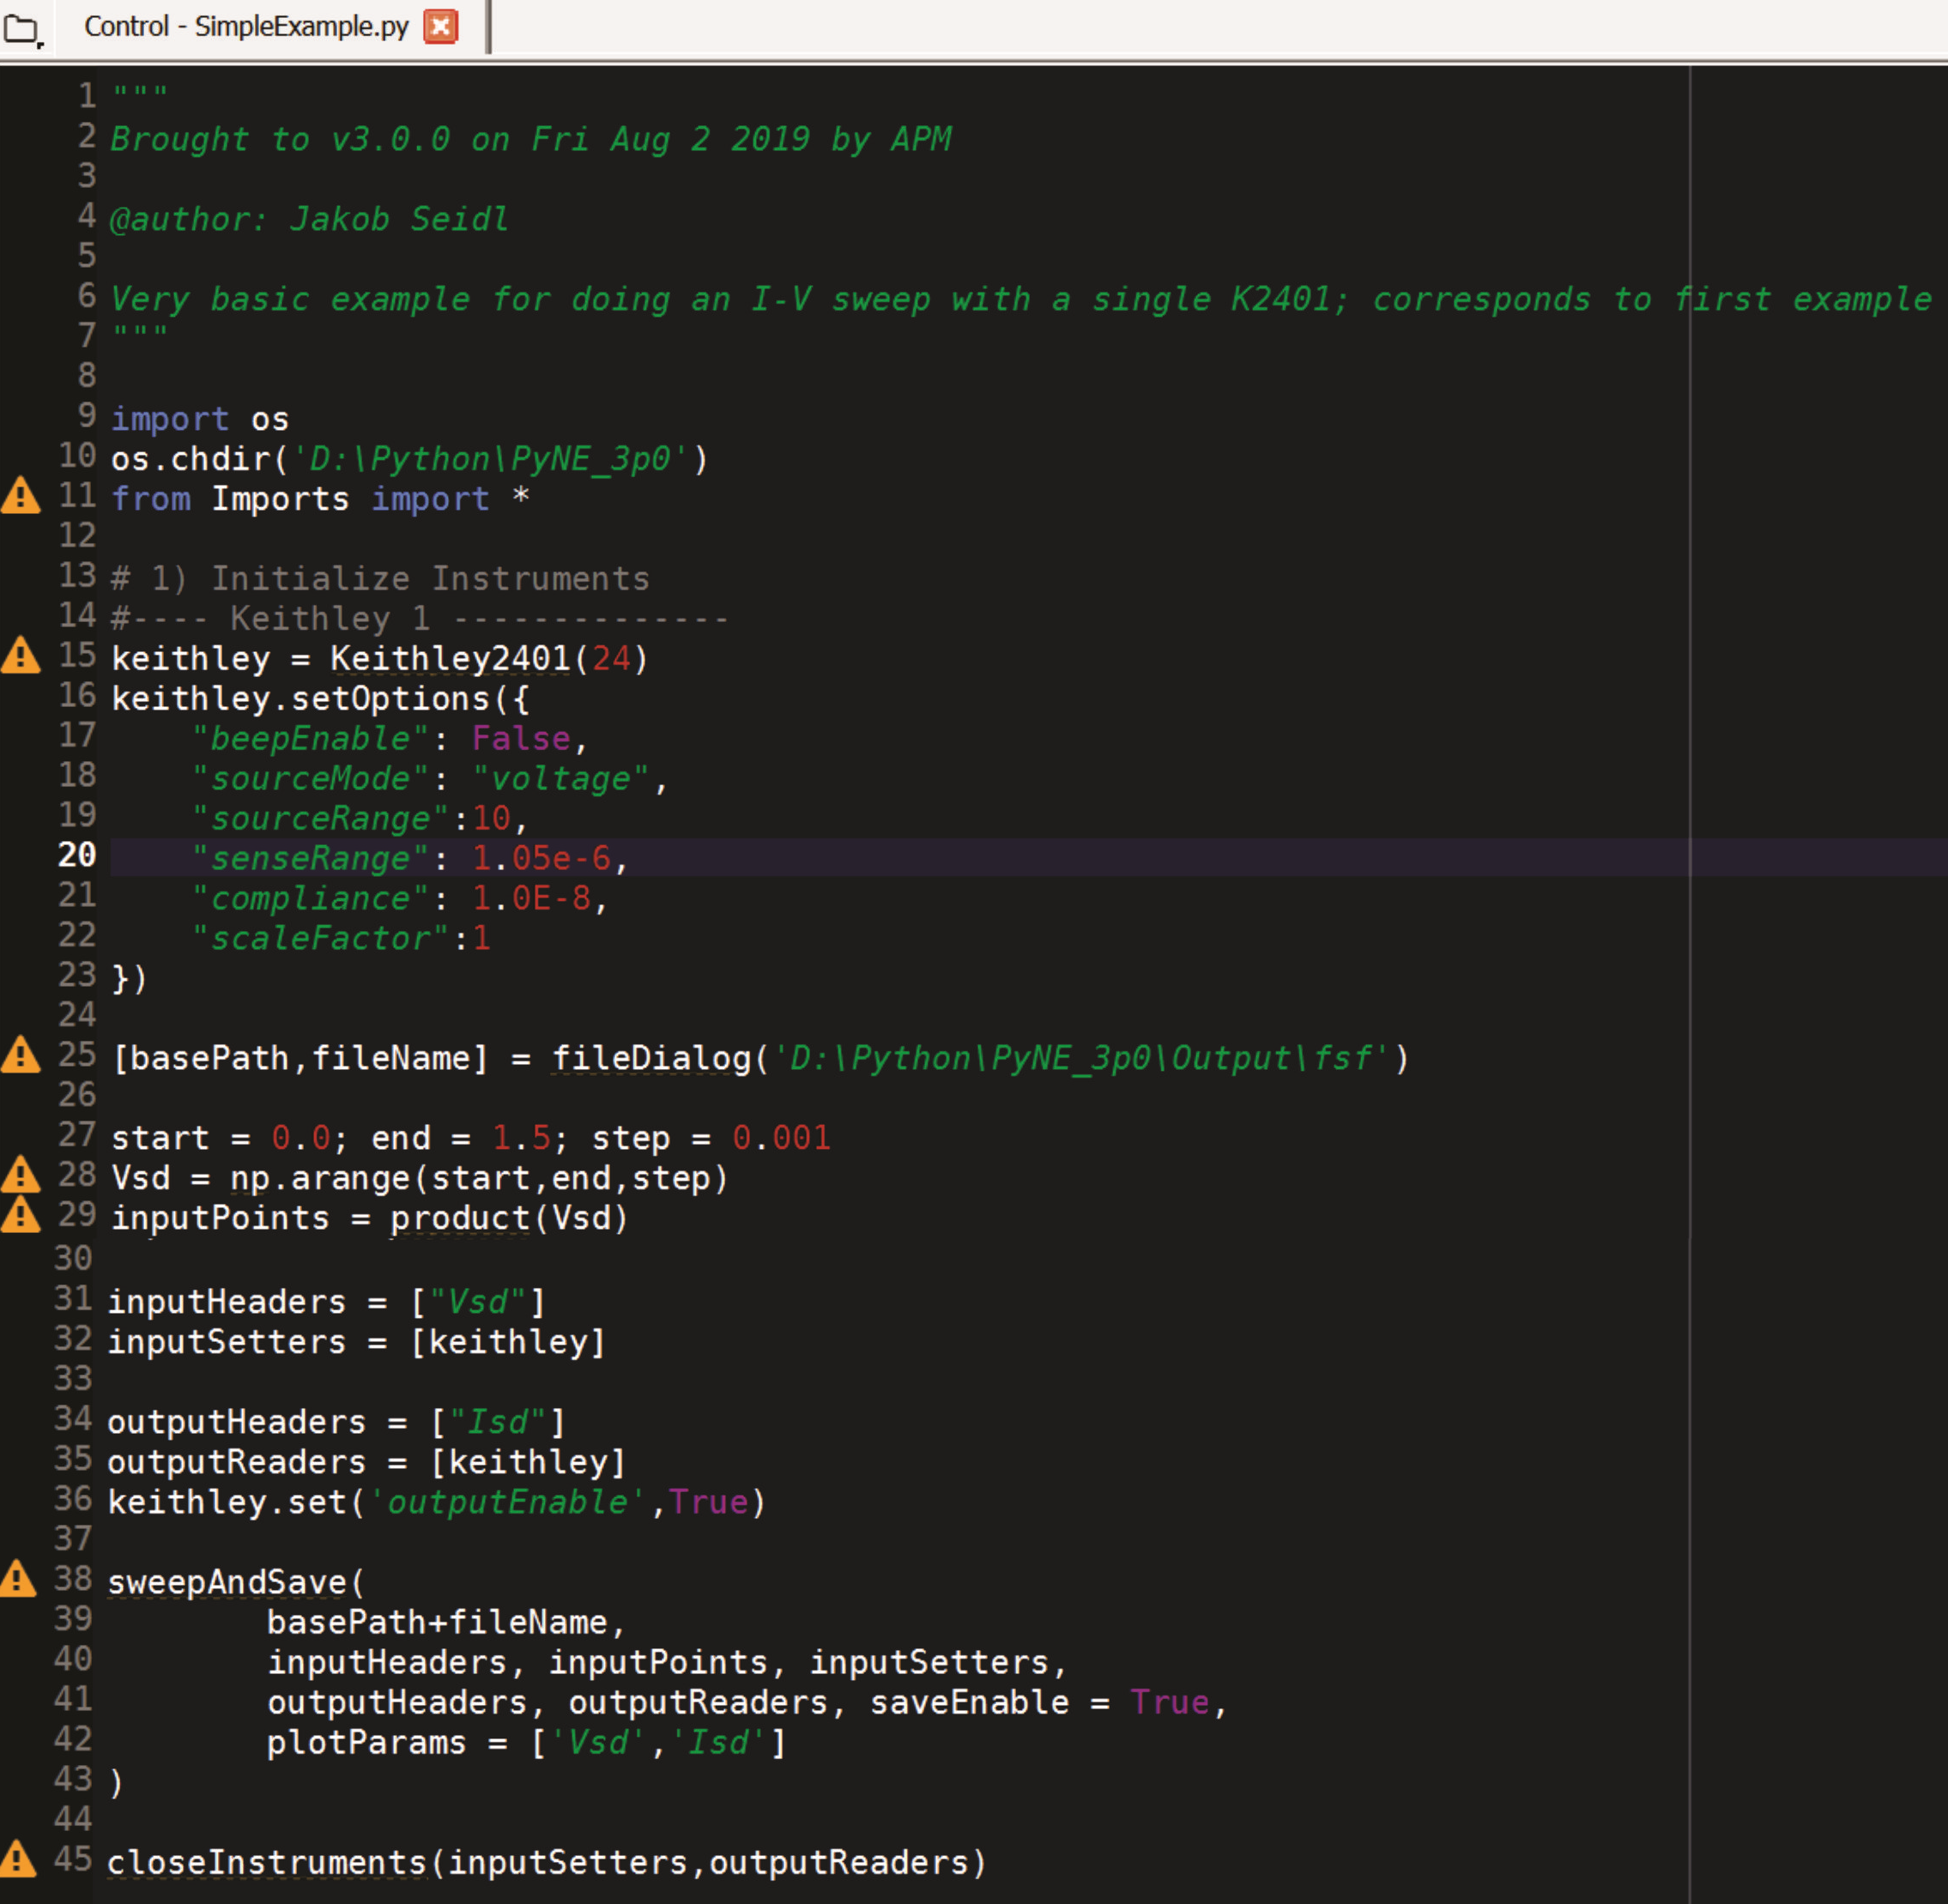
\includegraphics[width=16cm]{SimpleControl}
\caption{\textbf{Control workflow.} Lines 9-11 import the required functions. Lines 15-23 define an instrument and set the measurement options. Line 25 calls a GUI for selecting the results directory and file name. The array of data points we want to sweep over is defined in Lines 27-28 and converted into a suitable format in Line 29. Lines 31-36 show the setup of input and output headers $\textsf{\&}$ setters (see text). After the output of the SMU is enabled in Line 36, the main sweep function is called in Lines 38-43. Finally, all instrument connections are closed in Line 35.}
\label{Fig:SimpleControl}
\end{figure}

In the next section, the Keithley2401 instrument is defined and connected via the command:\\

\begin{verbatim}
keithley = Keithley2401(24)
\end{verbatim}

In pyNE, instruments themselves are `instances' of the corresponding instrument type, which are represented by `classes'. If you are reading this, you may well be new to Object Oriented Programming (OOP) as well as Python, so that last sentence will be unintelligible. This footnote\footnote{The links on OOP are: https://www.freecodecamp.org/news/object-oriented-programming-concepts-21bb035f7260/ and https://www.makeuseof.com/tag/object-oriented-programming-explained/} has some links on the basic concept of object oriented programming. This footnote\footnote{The link on basics of python is: https://swcarpentry.github.io/python-novice-inflammation/} has a good way to start learning the very basics of Python (albeit using Jupyter notebooks, but the syntax is very similar). So, assuming you now know at least the basic OOP concept, let's get back to it. Upon creation of an instrument instance, you only have to specify the instrument type (here Keithley2401) and GPIB address (here 24). You can create multiple instruments (instances) of the same type by repeating the above command using a different name and GPIB address, e.g., like this:\\

\begin{verbatim}
keithley1 = Keithley2401(24)
keithley2 = Keithley2401(11)
\end{verbatim}

There are only two instruments presently that violate this rule. The first is the `time' instrument, which takes as its argument the time interval rather than the GPIB. The second is the NI USB-6216, which takes as its argument the port number you want to control. The reason for this is that neither of these instruments is on the GPIB bus. More details on this in Section~2.\\

These instruments are instances of `classes' (see OOP footnote), which means you can use the rather convenient `dot notation', e.g., \texttt{keithley.goTo(0.0)}, to access the corresponding class functions, which are instrument operations, settings or parameters. Some of these functions are the most basic instrument functionalities you could access from their front panels, e.g., enable or disable output voltage. The software also provides some higher level functions that can execute sequences of low-level functions for you. In the example in Fig.~1.1, in Lines 16-23, we use the function below:\\

\begin{verbatim}
keithley.setOptions({
    "beepEnable": False,
    "sourceMode": "voltage",
    "sourceRange":10,
    "senseRange": 1.05e-6,
    "compliance": 1.0E-8,
    "scaleFactor":1
})
\end{verbatim}

to set a bunch of instrument options all at once. Every instrument has this function but the available options naturally vary from instrument to instrument. The options are formatted in python dictionary format, i.e., consist of a \texttt{`key'} with a corresponding \texttt{`value'}. A comprehensive list of all implemented options can be found in Section~2.\\
\\
Line 25 opens a short GUI (Graphical User Interface) dialog window, where a user specifies the desired base folder and filename for saving their data. These are saved in the variables `basePath' and `fileName', which can be overwritten manually via a later line in the code if needed, e.g., in order to give certain sweeps completely different filename structure.\\
\\
After all instruments are properly initialized, we can begin to define the parameter space we'd like to sweep through. The \textit{numpy arange}\footnote{\textit{numpy} is commonly imported as `np' in the python community and we stick to this convention.} is a convenient way of defining an equally spaced array ranging from a start to and end value\footnote{Note that np.arange by default excludes the endpoint - this is why Adam often prefers np.linspace, which has an endpoint = True/False option}, c.f. Lines 27-28. For a few discrete points, it might be better to use a simple python list like `Vsd = [0.2, 0.3, 0.5]' instead. The next line, Line 29, converts this newly defined array/list into the format required by the function that performs the actual sweep. It creates an \textit{itertools.product} `object' in the SweepFunction.py routine. For a single parameter sweep, like we do here, the product object will simply be a 1D array. However, when provided two or more inputs, this command will create a product array comprised of all the inputs. To give an example, say you'd like to perform a simple gatesweep measurement for a set of source-drain biases. You'd define the gatesweep range (Vg) using np.arange just like in the example code but additionally define `Vsd = [0.2, 0.3, 0.5]', for example. Then \texttt{InputPoints = product(Vsd,Vg)} would span your entire (2D) parameter space, i.e., do one full Vg sweep for Vsd$ = 0.2$~V, one for $0.3$~V and one for $0.5$~V. The order in which the inputs are placed matters, it governs the sweep order, so be careful about how this is assembled. The keyword \texttt{inputPoints} has been established as the keyword for the final array. This is just a name though and can be changed if needed.\\
\\
After initializing the instrument(s) and setting the sweep parameter space, we can now declare which of these instruments are going to actually do the sweep, i.e., set parameters (referred to as \textit{setters}) and which instruments will measure data (\textit{readers}). At the same time we also define how we want to call the parameters that are sourced or acquired. This is done via the \textit{headers} that exist for the swept variables (\textit{inputHeaders}) and measured data (\textit{outputHeaders}). If you have multiple instruments you define these via a simple list, e.g., inputSetters = [keithley,yokogawa]; the same holds for the corresponding headers. Make sure that the order in which the headers and setters are defined matches. The first setter will always be identified with the first header and so forth; avoid errors here since they will, at the least, create a lot of confusion in your data files. Some instruments return two values when measuring, e.g., lock-in amplifiers, you should use additional brackets [...] to denote this pair of variables, like this:\\

\begin{verbatim}
outputHeaders = [[Ix,Iy],GateLeakage]
outputReaders = [LockIn1,Keithley_Vg]
\end{verbatim}

Finally, after declaring input and output instruments and variables, we then pass all these variables to the main function \textit{sweepAndSave}, which performs the sweep:\\

\begin{verbatim}
sweepAndSave(
    basePath+fileName,
    inputHeaders, inputPoints, inputSetters,
    outputHeaders, outputReaders,saveEnable = True,breakCondition = breakCond,
    plotParams = ['Vsd','Isd']
)
\end{verbatim}

Let's quickly go through the input variables:\\

\begin{enumerate}
\item The full file path. Note that strings can just be added in python and thus basePath+fileName is just a string.
\item inputHeaders, inputPoints and inputSetters. These variables were defined above and specify instruments and values that are actively sourced.
\item outputHeaders, outputReaders. As defined above, these specify all instruments and quantities that are read/measured.
\item saveEnable is a boolean (True or False) that decides whether the obtained data will be saved (as .tsv, .mat and .png file) or not.
\item breakCondition = breakCondition is still in the making and not yet implemented. Please leave this out for now.
\item plotParams denotes the variables among inputHeaders and outputHeaders that you want to get plotted while measuring. Currently, you can only specify two pairs of variables, i.e., obtain two live plots. Note also that the first variable is always plotted on the \textit{x}-axis and must come from the \texttt{inputHeaders} while the second is on the \textit{y}-axis and should be chosen from the range of \texttt{outputHeaders}.
\end{enumerate}

The sweepAndSave() function will do the rest, i.e., slowly sweep all the setters to their initial sweep point (to avoid abrupt changes) and then carry out the sweep. Finally,\\

\begin{verbatim}
closeInstruments(inputSetters,outputReaders)
\end{verbatim}

will close the connection to all your instruments, as long as they are included in either inputSetter or outputReaders. You can also manually close any instrument by typing:\\

\begin{verbatim}
instrument.close()
\end{verbatim}

\section{A more complex example - combining measurements}
Having seen how to construct a simple measurement in our control file, it is time to move on to a more sophisticated example. Here we will combine \textit{$I_d$ vs. $V_{sd}$} measurement with a set of subsequent \textit{$I_d$ vs. $V_g$} gatesweeps.\\

\scriptsize
\begin{verbatim}
import os
os.chdir('D:\Python\PyNE_3p0')
from Imports import *

#----Keithley Vsd --------------
Ksd = Keithley2401(24)
Ksd.setOptions({
    "beepEnable": False,
    "sourceMode": "voltage",
    "sourceRange":1,
    "senseRange": 1.05e-5,
    "compliance": 1.0E-5,
    "scaleFactor":1
})

#---Keithley Vg -----------
KVg = Keithley2401(11)
KVg.setOptions({
    "beepEnable": False,
    "sourceMode": "voltage",
    "sourceRange":1,
    "senseRange": 1.05e-6,
    "compliance": 1.0E-7,
    "scaleFactor":1
})

#Electrometer
eMeter = Keithley6517A(20)
eMeter.setOptions({
    "autoRange":True,
    "senseRange":2E-6,
    "senseMode":"current",
})

[basePath,fileName] = fileDialog()

#Vsd array
start = -0.05; end = 0.5; step = 0.001 #Create a up and downsweep array
VsdUp = np.arange(start, end, step) #Only the upsweep
VsdDown = np.arange(end, start-step, -step)
VsdUpDown = np.concatenate((VsdUp, VsdDown)) #np.concatenate() fuses two arrays to one

#Gatesweep array, Vg
start = 0.0; end = 1.4; step = 0.005 #Create a up and downsweep array
Vg = np.concatenate(( #np.concatenate() fuses two arrays to one
        np.arange(start, end, step),
        np.arange(end, start-step, -step)
))

#--------------Headers and setters for IV curves
inputHeaders = ["Vsd"]
inputSetters = [Ksd]
outputHeaders = ["Id","Idrough"]
outputReaders = [eMeter,Ksd]
Ksd.set('outputEnable',True)
for i in range(3): # 3 Vsd sweeps from -0.05 -> 0.05 V
    inputPoints = product(VsdUpDown)
    sweepAndSave(
            basePath+fileName,
            inputHeaders, inputPoints, inputSetters,
            outputHeaders, outputReaders,saveEnable = True,
            plotParams = ['Vsd','Id']
    )
Ksd.goTo(0.05,delay=0.001) # since we stop the sweep at -0.05 V we go to 0.05 V manually

#--------------Headers and setters for Vg curves
inputHeaders = ["Vg"]
inputSetters = [KVg]
outputHeaders = ["Id","Ileak","Idrough"]
outputReaders = [eMeter,KVg,Ksd]
for i in range(5): # do 5 full gatesweeps from 0 to 1.4 V
    inputPoints = product(Vg)
    sweepAndSave(
            basePath+fileName,
            inputHeaders, inputPoints, inputSetters,
            outputHeaders, outputReaders,saveEnable = True,
            plotParams = ['Vg','Id','Vg','Ileak']
    )

Ksd.goTo(0.00,delay=0.001)

closeInstruments(inputSetters,outputReaders)
\end{verbatim}
\normalsize

Here, we import three instruments: two Keithley2401 source-measure units (SMUs) and one Keithley6517A electrometer. After setting their options, we define arrays for both the gate voltage $V_{\mathrm{g}}$ and the source-drain bias $V_{\mathrm{sd}}$. The \texttt{np.concatenate()} function is used to join two arrays into one. This allows for up and downsweeps using just one array or using a higher point-spacing in certain parts of the sweep than in others.\footnote{For example, you could have a coarse spacing in the uninteresting regions of a gatesweep and a fine resolution in an interesting region.} Note that the headers and setters must be defined separately for each measurement, since different instruments are sourcing the voltages/currents in each of these measurements. You might also want to measure a separate set of variables, and name them differently, and this is possible with this structure.\\
\\
Two last things we'd like to draw your attention to:\\
Any setter instrument can be swept to any (sensible) value using:\\

\begin{verbatim}
instrument.goTo(targetValue,stepsize,delay)
\end{verbatim}

This is the same command we use before performing the gate sweep in order to sweep the source-drain bias back from $-0.05$~V to $0.05$~V. Note also the use of \textit{for loops} in this script. These provide a very simple control over how many times we'd like to perform a sweep. One could in principle combine \textit{for} and \textit{while} loops with different conditions based on measurement outcomes to creating more sophisticated measurement routines, e.g., sequence of repeated measurements that self-terminates once one of the parameters crosses a threshold.\\



